% !TeX program = xelatex
\documentclass[11pt,a4paper]{article}

% -----------------------------------------------------------------------------
% Page layout and typography
% -----------------------------------------------------------------------------
\usepackage[a4paper,margin=1in,headheight=14pt]{geometry}
\usepackage[T1]{fontenc}
\usepackage{lmodern}
\usepackage[scaled=0.92]{helvet}
\usepackage{setspace}
\setstretch{1.08}
\usepackage{parskip}
\usepackage{titlesec}
\usepackage{fancyhdr}
\usepackage{needspace}
\emergencystretch=2em

% -----------------------------------------------------------------------------
% Mathematics, tables, boxes, figures, code
% -----------------------------------------------------------------------------
\usepackage{amsmath,amssymb,bm,mathtools}
\usepackage{booktabs,tabularx,longtable,array,multirow}
\usepackage[table]{xcolor}
\usepackage{graphicx}
\usepackage{caption}
\usepackage{enumitem}
\usepackage[most]{tcolorbox}
\usepackage{listings}
\usepackage{hyperref}
\usepackage[nameinlink,noabbrev]{cleveref}

\graphicspath{{../assets/}{./}}

% -----------------------------------------------------------------------------
% Colors and hyperref
% -----------------------------------------------------------------------------
\definecolor{TutorialBlue}{HTML}{1F4E79}
\definecolor{SoftBlue}{HTML}{EAF3F8}
\definecolor{SoftGreen}{HTML}{ECF8F1}
\definecolor{SoftYellow}{HTML}{FFF7E6}
\definecolor{SoftRed}{HTML}{FDEDEC}
\definecolor{RuleGrey}{HTML}{D9E2EC}
\definecolor{CodeBack}{HTML}{F7F7F9}
\definecolor{CodeFrame}{HTML}{D6D6D6}
\definecolor{CodeKeyword}{HTML}{1F4E79}
\definecolor{CodeComment}{HTML}{5F6F52}

\hypersetup{
  colorlinks=true,
  linkcolor=TutorialBlue,
  citecolor=TutorialBlue,
  urlcolor=TutorialBlue,
  pdftitle={Optimal Control, Differential Games, Hybrid Control, and Games on Networks},
  pdfauthor={Lu-Xing Yang},
  pdfsubject={Self-contained tutorial note},
  pdfkeywords={optimal control, differential games, hybrid control, impulse control, networks, Python}
}

% -----------------------------------------------------------------------------
% Heading and page styles
% -----------------------------------------------------------------------------
\titleformat{\section}{\Large\bfseries\sffamily\color{TutorialBlue}}{\thesection}{0.7em}{}
\titleformat{\subsection}{\large\bfseries\sffamily\color{TutorialBlue}}{\thesubsection}{0.7em}{}
\titleformat{\subsubsection}{\normalsize\bfseries\sffamily\color{TutorialBlue}}{\thesubsubsection}{0.7em}{}
\titlespacing*{\section}{0pt}{1.0em}{0.45em}
\titlespacing*{\subsection}{0pt}{0.8em}{0.35em}
\titlespacing*{\subsubsection}{0pt}{0.6em}{0.25em}

\pagestyle{fancy}
\fancyhf{}
\lhead{\small\sffamily Optimal Control, Games, and Hybrid Control}
\rhead{\small\sffamily \thepage}
\renewcommand{\headrulewidth}{0.4pt}
\renewcommand{\footrulewidth}{0pt}

% -----------------------------------------------------------------------------
% Table and list helpers
% -----------------------------------------------------------------------------
\renewcommand{\arraystretch}{1.22}
\newcolumntype{Y}{>{\raggedright\arraybackslash}X}
\newcolumntype{L}[1]{>{\raggedright\arraybackslash}p{#1}}
\setlist[itemize]{leftmargin=1.35em,itemsep=0.20em,topsep=0.25em}
\setlist[enumerate]{leftmargin=1.55em,itemsep=0.20em,topsep=0.25em}

% -----------------------------------------------------------------------------
% Boxes
% -----------------------------------------------------------------------------
\tcbset{
  enhanced,
  sharp corners,
  boxrule=0.6pt,
  left=6pt,right=6pt,top=5pt,bottom=5pt,
  before skip=0.55em,after skip=0.75em
}
\newtcolorbox{definitionbox}[1]{colback=SoftBlue,colframe=TutorialBlue,title=\textbf{#1}}
\newtcolorbox{examplebox}[1]{colback=SoftGreen,colframe=green!45!black,title=\textbf{#1}}
\newtcolorbox{cautionbox}[1]{colback=SoftYellow,colframe=orange!80!black,title=\textbf{#1}}
\newtcolorbox{sourcebox}[1]{colback=SoftRed,colframe=red!60!black,title=\textbf{#1}}

% -----------------------------------------------------------------------------
% Listings
% -----------------------------------------------------------------------------
\lstdefinestyle{pythonstyle}{
  language=Python,
  basicstyle=\scriptsize\ttfamily,
  keywordstyle=\color{CodeKeyword}\bfseries,
  commentstyle=\color{CodeComment}\itshape,
  stringstyle=\color{purple!70!black},
  showstringspaces=false,
  breaklines=true,
  breakatwhitespace=false,
  keepspaces=true,
  columns=fullflexible,
  frame=single,
  rulecolor=\color{CodeFrame},
  backgroundcolor=\color{CodeBack},
  numbers=left,
  numberstyle=\tiny\color{gray},
  xleftmargin=2.0em,
  framexleftmargin=1.6em,
  tabsize=4,
  captionpos=b
}
\lstset{style=pythonstyle}

% -----------------------------------------------------------------------------
% Math shortcuts
% -----------------------------------------------------------------------------
\newcommand{\R}{\mathbb{R}}
\newcommand{\dd}{\,\mathrm{d}}
\newcommand{\argmax}{\operatorname*{arg\,max}}
\newcommand{\argmin}{\operatorname*{arg\,min}}
\newcommand{\Proj}{\operatorname{Proj}}
\newcommand{\T}{\mathsf{T}}

\begin{document}

% -----------------------------------------------------------------------------
% Title page
% -----------------------------------------------------------------------------
\begin{titlepage}
\centering
\vspace*{1.5cm}
{\sffamily\bfseries\Huge\color{TutorialBlue} Optimal Control, Differential Games, Hybrid Control, and Games on Networks\par}
\vspace{0.5cm}
{\sffamily\Large A Self-Contained English Tutorial Note with Degree-Level and Node-Level Examples\par}
\vspace{0.8cm}
{\large Lu-Xing Yang\par}
\vspace{0.8cm}
{\large Created from my research experience in optimal control, differential games, hybrid/impulsive control, and cyber/network-security applications\par}
\vspace{0.35cm}
{\large Informed by publications in IEEE TIFS, TDSC, TSMC, TNSE, TCSS, and related journals\par}
\vspace{0.35cm}
{\large Tutorial Python files: \texttt{simple\_degree\_k\_control.py} and \texttt{network\_control\_examples.py}\par}
\vfill
\begin{tcolorbox}[width=0.86\textwidth,colback=SoftBlue,colframe=TutorialBlue]
\textbf{Purpose.} This note starts from controlled dynamical systems and develops optimal control, differential games, and hybrid/impulsive control in one coherent framework. It is written for propagation, defense, and intervention problems on networks. The mathematical sections introduce the state equation, payoff, Hamiltonian, PMP, HJB/HJI viewpoint, Nash equilibrium conditions, impulse jumps, and hybrid strategies. The computational sections give a simple degree-$k$ example first and then a main tutorial script for degree-level games, node-level adjacency-matrix models, and hybrid/impulsive simulations. The degree-level workflow always computes $N_k$, $P(k)$, and $\langle k\rangle$ from the input network before solving models indexed by degree class $k$.
\end{tcolorbox}
\vfill
{\large \today\par}
\end{titlepage}

\tableofcontents
\newpage

% -----------------------------------------------------------------------------
\section{How to Read This Handout}
% -----------------------------------------------------------------------------

This handout follows a layered structure. First, it defines a controlled dynamical system. Second, it formulates an optimal control problem for one decision maker. Third, it extends the same logic to two or more strategic decision makers, producing a differential game. Fourth, it adds discrete state jumps and event decisions, producing impulse and hybrid control/game models. Finally, it connects the mathematics to degree-level and node-level propagation models on networks and to runnable Python implementation.

\begin{definitionbox}{Core questions}
\begin{itemize}
  \item \textbf{Optimal control}: what should one controller do over time to maximize benefit or minimize cost?
  \item \textbf{Differential game}: what should each player do when the system state is jointly affected by all players and their objectives may conflict?
  \item \textbf{Impulse control/game}: when and how should a player apply instantaneous actions that cause state jumps?
  \item \textbf{Hybrid control/game}: how should continuous-time controls and discrete impulses/switching decisions be combined?
  \item \textbf{Degree-level versus node-level networks}: should we group nodes by type/degree, or track every node and use the full adjacency matrix?
\end{itemize}
\end{definitionbox}

\begin{table}[h!]
\centering
\caption{A layered view of the tutorial note.}
\begin{tabularx}{\textwidth}{L{2.9cm}L{3.5cm}Y Y}
\toprule
\textbf{Layer} & \textbf{Mathematical object} & \textbf{Typical question} & \textbf{Network example} \\
\midrule
Continuous dynamics & $\dot{x}=f(x,u,t)$ & How does the state evolve under continuous effort? & Patch rate, recovery effort, attack rate over time \\
Optimal control & $\max_u J(u)$ subject to dynamics & What is the best control for one decision maker? & Defender allocates patching to reduce malware \\
Differential game & $\max_{u_i} J_i(u_i,u_{-i})$ for each player & What is a Nash or Stackelberg equilibrium? & Attacker increases spread; defender suppresses spread \\
Impulse control & $x(t_l^+) = x(t_l^-) + g(x(t_l^-),v_l)$ & When should discrete interventions be applied? & Emergency cleanup, forced password reset, public correction campaign \\
Hybrid control/game & Continuous dynamics plus impulses/switches & How should continuous and discrete decisions be combined? & Routine monitoring plus occasional large-scale response \\
\bottomrule
\end{tabularx}
\end{table}



\begin{definitionbox}{Notation conventions used throughout the note}
The same mathematical object can be written differently in different communities. This note uses the following convention unless explicitly stated otherwise.
\begin{center}
\begin{tabularx}{0.96\textwidth}{L{2.8cm}Y}
\toprule
\textbf{Symbol} & \textbf{Meaning} \\
\midrule
$T$ & finite time horizon; the control/game runs on $[0,T]$. \\
$x(t)\in\mathbb{R}^n$ & state vector. In node-level models, $x_i(t)$ is the infection, compromise, belief, or risk level at node $i$. \\
$u(t),v(t)$ & controls. In games, different symbols usually belong to different players. \\
$A=[a_{ij}]$ & adjacency matrix. In this note, $(A x)_i=\sum_j a_{ij}x_j$ is the pressure on node $i$ from its neighbors. \\
$F,L$ & running payoff or running loss. We use maximization with $F$ and minimization with $L$. \\
$H$ & Hamiltonian. For games there is one Hamiltonian per player. \\
$\lambda(t)$ & adjoint or costate. It is solved backward in time and acts as a shadow value of the state. \\
$t_l,v_l$ & impulse time and impulse magnitude at event $l$. \\
\bottomrule
\end{tabularx}
\end{center}
\end{definitionbox}

% -----------------------------------------------------------------------------
\section{Dynamic Systems and Network Propagation Models}
% -----------------------------------------------------------------------------

A dynamic system describes how a state changes over time. In cybersecurity, information diffusion, epidemiology, and social network analysis, the state may measure infection, compromise, awareness, rumor belief, or defense status. A control modifies the state equation. A game appears when two or more decision makers control the same system with different objectives.

\subsection{State, Control, and Objective}

Let the time horizon be $[0,T]$. Let $x(t)\in\R^n$ be the state vector and $u(t)\in U$ be the control. A deterministic continuous-time controlled system is written as
\begin{equation}
  \dot{x}(t)=f(x(t),u(t),t),\qquad x(0)=x_0,\qquad 0\leq t\leq T.
  \label{eq:basic-dynamics}
\end{equation}
The controller usually optimizes a cumulative payoff or cost. A maximization form is
\begin{equation}
  J(u)=\Phi(x(T))+\int_0^T F(x(t),u(t),t)\dd t.
  \label{eq:basic-objective}
\end{equation}
Here $F$ is the running payoff and $\Phi$ is the terminal payoff. In a minimization formulation, $F$ is often a running cost such as infection loss plus control cost.


\subsection{Degree-Level Models}

\needspace{8\baselineskip}
\begin{definitionbox}{Degree-level state means degree-indexed state}
A degree-level model should not be implemented as a single scalar compartmental SIR/SIS model unless the network is being ignored. In a network-aware degree-level model, the first step is to compute the degree classes from the input graph. If $N_k$ is the number of nodes with degree $k$ and $n$ is the total number of nodes, then
\begin{equation}
  P(k)=\frac{N_k}{n},
  \qquad
  \bar{k}=\frac{1}{n}\sum_{i=1}^n k_i=\sum_k kP(k).
  \label{eq:degree-distribution}
\end{equation}
The state is then arranged as
\begin{equation}
\begin{aligned}
  x(t)&=\bigl(x_k(t)\bigr)_{k\in\mathcal{K}},\qquad
  \mathcal{K}=\{k:N_k>0\},\\
  x_k(t)&=\text{infected/compromised fraction among degree-}k\text{ nodes}.
\end{aligned}
  \label{eq:degree-state-vector}
\end{equation}
\end{definitionbox}

A common heterogeneous mean-field infection pressure is
\begin{equation}
  \Theta(t)=\frac{\sum_{k\in\mathcal{K}} kP(k)x_k(t)}{\langle k\rangle},
  \label{eq:theta-degree}
\end{equation}
where $P(k)$ is the degree distribution and $\langle k\rangle=\bar{k}$ is the average degree. A controlled degree-level SIS-style model is
\begin{equation}
  \dot{x}_k(t)=\beta k(1-x_k(t))\Theta(t)-\bigl(\delta+u_k(t)\bigr)x_k(t),
  \qquad k\in\mathcal{K}.
  \label{eq:degree-sis}
\end{equation}
The implementation therefore stores one state and one control trajectory per observed degree value. For example, if the input network has degree classes $\mathcal{K}=\{2,3,4,7\}$, then the model state is $(x_2,x_3,x_4,x_7)$, not $(S,I,R)$.

The code also supports class-specific physical and economic parameters.  With susceptibility $s_k$, infectivity $\iota_k$, recovery $\delta_k$, and row-stochastic mixing $M_{k\ell}$, the heterogeneous pressure is
\[
  \lambda_k(t)=s_k k\sum_{\ell\in\mathcal{K}} M_{k\ell}\iota_\ell x_\ell(t),
  \qquad
  \dot{x}_k(t)=(1-x_k(t))\lambda_k(t)-(\delta_k+u_k(t))x_k(t).
\]
Scalar inputs are explicitly broadcast by \texttt{cybercontrol.heterogeneity}, so the homogeneous model remains a special case.

In the tutorial code, \texttt{compute\_degree\_distribution} returns the observed degree values, counts $N_k$, probabilities $P(k)$, and average degree $\langle k\rangle$. For directed networks, one must also decide what ``degree'' means. The code exposes a \texttt{degree\_mode} option: row degree counts incoming influencers under the convention $\dot{x}=f(Ax)$, column degree counts outgoing influence, total degree adds both, and undirected degree ignores orientation.

Degree-level models are compact and interpretable. They are useful when the network is large or only statistical network information is available. Their limitation is that they lose fine node-level structure: which node is connected to which node, which node is high value, and where attacks or defenses should be targeted.

\subsection{Node-Level Models}

A node-level model tracks each node. Let $A=[a_{ij}]$ be the adjacency matrix. Let $x_i(t)$ be the probability or intensity that node $i$ is infected or compromised. A standard controlled node-level model is
\begin{equation}
  \dot{x}_i(t)=\beta(1-x_i(t))\sum_{j=1}^n a_{ij}x_j(t)-\bigl(\delta+u_i(t)\bigr)x_i(t),\qquad i=1,\dots,n.
  \label{eq:node-sis}
\end{equation}
Here $\beta$ is the propagation rate, $\delta$ is the natural recovery/removal rate, and $u_i(t)$ is node-specific defense effort. This model explicitly uses network connectivity and supports targeted control. The cost is computational: the state dimension grows with $n$, and the adjoint or HJB equation becomes harder as the network grows.

\subsection{From a Real Network Dataset to the Adjacency Matrix}
\label{subsec:real-network-to-adj}

Real network datasets are often not distributed as adjacency matrices. They are usually stored as an \emph{edge list}: each row records a connection such as
\begin{center}
\texttt{source target}\qquad or \qquad \texttt{source,target,weight}.
\end{center}
To use such a dataset in this tutorial, the code first parses the full input network and computes the empirical degree distribution $N_k$, $P(k)$, and $\langle k\rangle$. It then optionally converts a smaller high-degree induced subgraph into a dense adjacency matrix $A$ for node-level PMP/game examples. Thus, degree-level models can use the full-network degree distribution even when node-level examples use a reduced adjacency matrix for computational clarity. The conversion is conceptually simple but important, because mistakes in node indexing, direction, self-loops, or normalization can change the dynamics substantially.

\begin{examplebox}{Edge list to adjacency matrix: practical workflow}
\begin{enumerate}
  \item \textbf{Read edges.} Parse each line as $(\text{source},\text{target})$ or $(\text{source},\text{target},\text{weight})$.
  \item \textbf{Relabel nodes.} Map arbitrary node labels such as account IDs or IP addresses to integer indices $0,\dots,n-1$.
  \item \textbf{Choose directed or undirected.} For an undirected contact graph, set both $a_{ij}$ and $a_{ji}$. For a directed influence graph, keep the edge direction.
  \item \textbf{Remove self-loops and invalid weights.} Most SIS/SIR-style propagation examples assume $a_{ii}=0$ and nonnegative weights.
  \item \textbf{Normalize if needed.} Divide by maximum degree, row sums, or spectral radius to keep propagation probabilities numerically stable.
  \item \textbf{Reduce size if needed for node-level computation.} Full node-level PMP uses dense adjoint/Jacobian calculations. For large datasets, first keep a subgraph such as the top-degree 30--200 nodes, a community, or a sampled ego-network. The degree-level distribution $P(k)$ can still be computed from the full input network before this reduction.
\end{enumerate}
\end{examplebox}

The tutorial code implements this workflow in the single-file functions \texttt{load\_network}, \texttt{graph\_to\_model\_matrix}, and \texttt{degree\_distribution\_from\_graph}. The convention used by the dynamics is
\begin{equation}
  \text{infection pressure on node } i=(Ax)_i=\sum_{j=1}^n a_{ij}x_j.
\end{equation}
Thus, for a directed edge ``source influences target'', the code places the edge weight in the matrix row for the target and the matrix column for the source. For an undirected graph, it symmetrizes the matrix.


\begin{lstlisting}[caption={Minimal example: load an edge-list dataset, compute the degree distribution, and run degree-level and node-level models.}]
from network_control_examples import (
    build_parser,
    load_network,
    degree_distribution_from_graph,
    solve_degree_control,
    solve_node_control,
)

args = build_parser().parse_args([
    "--edge-list", "data/edges.txt",
    "--max-nodes", "30",        # only reduces the node-level matrix
    "--degree-mode", "undirected",
])

network = load_network(args)
D = degree_distribution_from_graph(network.full_graph, mode=args.degree_mode)
A = network.A

# Degree-level workflow: columns are observed degree classes k.
degree_result = solve_degree_control(D)

# Node-level workflow: use the dense simulation adjacency matrix A.
node_result = solve_node_control(A)
\end{lstlisting}

\begin{cautionbox}{Scaling warning}
A real network can contain thousands or millions of nodes. The node-level PMP examples in this note intentionally use dense matrices so that the mathematics is transparent. For large datasets, use a subgraph, degree-level aggregation, sparse linear algebra, direct simulation with heuristic controls, or other approximate methods. The full HJB equation is even more expensive because its value function lives on the whole state space.
\end{cautionbox}


\begin{table}[h!]
\centering
\caption{Degree-level versus node-level models.}
\begin{tabularx}{\textwidth}{L{3.1cm}YY}
\toprule
\textbf{Aspect} & \textbf{Degree-level model} & \textbf{Node-level model} \\
\midrule
State dimension & Number of degree classes or compartments & Number of nodes times number of compartments \\
Network information & Degree distribution or mixing pattern & Full adjacency matrix or contact graph \\
Best use case & Large networks, aggregate analysis, early theory & Small/medium networks, targeted control, simulation \\
Main weakness & Less precise for targeted interventions & High dimensionality and possible data requirements \\
\bottomrule
\end{tabularx}
\end{table}

% -----------------------------------------------------------------------------
\section{Optimal Control: Single Decision Maker}
% -----------------------------------------------------------------------------

Optimal control is the single-player foundation. It asks for a time-dependent control strategy $u^*(t)$ that optimizes an objective while satisfying the system dynamics. This is the natural starting point for differential games.

\subsection{General Model}

\begin{align}
  \max_{u(\cdot)\in U} \quad & J(u)=\int_0^T F(x(t),u(t),t)\dd t, \label{eq:oc-obj}\\
  \text{s.t.}\quad & \dot{x}(t)=f(x(t),u(t),t),\qquad x(0)=x_0. \label{eq:oc-state}
\end{align}
In a minimization problem, the same structure applies after changing the sign of the objective. For example, minimizing infection and control cost is equivalent to maximizing the negative of that cost.

\subsection{Hamiltonian and Pontryagin Maximum Principle}

The Hamiltonian combines the immediate payoff and the effect of the control on future state evolution. For a maximization problem,
\begin{equation}
  H(x,u,\lambda,t)=F(x,u,t)+\lambda^{\T}f(x,u,t).
  \label{eq:oc-hamiltonian}
\end{equation}
The adjoint variable $\lambda(t)$ is a shadow value of the state: it measures how a small change in the state affects future payoff. Under standard regularity assumptions, a candidate optimum must satisfy the following necessary conditions:
\begin{align}
  \dot{x}^*(t)&=f(x^*(t),u^*(t),t), \qquad x^*(0)=x_0, \label{eq:oc-pmp-state}\\
  \dot{\lambda}^*(t)&=-\frac{\partial H}{\partial x}(x^*(t),u^*(t),\lambda^*(t),t), \qquad \lambda^*(T)=0, \label{eq:oc-pmp-adjoint}\\
  u^*(t)&\in\argmax_{u\in U}H(x^*(t),u,\lambda^*(t),t). \label{eq:oc-pmp-control}
\end{align}
These equations form a two-point boundary value problem: the state has an initial condition, while the adjoint has a terminal condition. This is why forward-backward sweep is commonly used.

\begin{cautionbox}{What PMP does and does not prove}
PMP gives necessary conditions under regularity assumptions. It does not automatically prove that a computed control is globally optimal. In practice, one should compare the computed policy with baselines, test sensitivity, and report convergence residuals.
\end{cautionbox}

\subsection{Forward-Backward Sweep}

Forward-backward sweep is an iterative numerical method for solving PMP optimality systems. The idea is simple but powerful: guess the control, simulate the state forward, simulate the adjoint backward, update the control from the Hamiltonian condition, and repeat.

\begin{examplebox}{Generic forward-backward sweep}
\begin{enumerate}
  \item Initialize $u^{(0)}(t)$, usually zero, constant, or a simple heuristic.
  \item Forward step: solve $\dot{x}=f(x,u^{(r)},t)$ from $t=0$ to $T$.
  \item Backward step: solve $\dot{\lambda}=-H_x$ from $t=T$ to $0$ using the state trajectory.
  \item Control update: compute $u_{\mathrm{new}}(t)=\argmax H$ or $\argmin H$ depending on the formulation.
  \item Relaxation: set $u^{(r+1)}=\theta u_{\mathrm{new}}+(1-\theta)u^{(r)}$ to improve stability.
  \item Stop when the control and state changes are below a tolerance, or after a maximum number of iterations.
\end{enumerate}
\end{examplebox}

\begin{lstlisting}[caption={Forward-backward sweep pseudocode.}]
for iteration in range(max_iter):
    x = forward_simulate(control)
    lambda_adj = backward_simulate(x, control)
    candidate_control = pointwise_hamiltonian_optimizer(x, lambda_adj)
    control = theta * candidate_control + (1 - theta) * control
    if convergence_is_satisfactory:
        break
\end{lstlisting}

\subsection{Important Practical Cautions}

\begin{itemize}
  \item Forward-backward sweep may fail to converge if the model is stiff, the horizon is long, the control bounds are sharp, or the initial guess is poor.
  \item A computed control should be compared with no control, constant control, greedy control, random timing, or heuristic resource allocation.
  \item For high-dimensional node-level systems, HJB is usually infeasible because the value function depends on every state dimension.
\end{itemize}

% -----------------------------------------------------------------------------
\section{Differential Games: Multiple Strategic Decision Makers}
% -----------------------------------------------------------------------------

A differential game is an optimal control problem with multiple players. The same state is affected by multiple controls, and each player has its own payoff. In cybersecurity, the players may be an attacker and a defender. In opinion or propaganda dynamics, they may be competing campaigns. In malware and patching, one player may inject infection effort while the other allocates repair or backup resources.

\subsection{General Two-Player Nonzero-Sum Open-Loop Nash Game}

Let player 1 choose $u(t)$ and player 2 choose $v(t)$. The system is
\begin{equation}
  \dot{x}(t)=f(x(t),u(t),v(t),t),\qquad x(0)=x_0.
  \label{eq:dg-state}
\end{equation}
Each player has a payoff:
\begin{align}
  J_1(u,v)&=\int_0^T F_1(x(t),u(t),v(t),t)\dd t,\label{eq:j1}\\
  J_2(u,v)&=\int_0^T F_2(x(t),u(t),v(t),t)\dd t.\label{eq:j2}
\end{align}
An open-loop Nash equilibrium $(u^*,v^*)$ satisfies
\begin{align}
  J_1(u^*,v^*)&\geq J_1(u,v^*) \qquad \text{for all admissible }u,\label{eq:nash1}\\
  J_2(u^*,v^*)&\geq J_2(u^*,v) \qquad \text{for all admissible }v.\label{eq:nash2}
\end{align}
Open-loop means each control is a function of time, usually computed before the game starts. Feedback strategies depend on the current state $x(t)$, but solving feedback differential games often requires HJB or Hamilton-Jacobi-Isaacs equations, which are much harder in high dimensions.

\subsection{Classification of Differential Games}

\begin{table}[h!]
\centering
\caption{Common classifications of differential games.}
\begin{tabularx}{\textwidth}{L{3.0cm}L{3.2cm}Y}
\toprule
\textbf{Dimension} & \textbf{Main types} & \textbf{Meaning for applications} \\
\midrule
Payoff relation & Zero-sum; nonzero-sum & Zero-sum is pure conflict; nonzero-sum allows asymmetric or partially aligned objectives. \\
State evolution & Deterministic; stochastic & Deterministic models are easier; stochastic models handle random disturbances and uncertainty. \\
Decision order & Nash; Stackelberg & Nash players move simultaneously; Stackelberg has leader-follower structure. \\
Information structure & Open-loop; feedback; sampled-data & Open-loop uses time plans; feedback observes state; sampled-data updates at discrete observation times. \\
Action type & Continuous; impulse; hybrid & Continuous changes derivatives; impulse causes jumps; hybrid combines both. \\
\bottomrule
\end{tabularx}
\end{table}

\subsection{PMP for an Open-Loop Nash Differential Game}

For each player $i$, define a player-specific Hamiltonian:
\begin{equation}
  H_i(x,u,v,\lambda_i,t)=F_i(x,u,v,t)+\lambda_i^{\T}f(x,u,v,t),\qquad i=1,2.
  \label{eq:dgame-ham}
\end{equation}
A candidate open-loop Nash equilibrium must satisfy the state equation, one adjoint system for each player, and one pointwise best-response condition for each player:
\begin{align}
  \dot{\lambda}_i(t)&=-\frac{\partial H_i}{\partial x}(x^*(t),u^*(t),v^*(t),\lambda_i(t),t),\qquad \lambda_i(T)=0,\quad i=1,2,\label{eq:dg-adjoint}\\
  u^*(t)&\in\argmax_u H_1(x^*(t),u,v^*(t),\lambda_1(t),t),\label{eq:dg-u}\\
  v^*(t)&\in\argmax_v H_2(x^*(t),u^*(t),v,\lambda_2(t),t).\label{eq:dg-v}
\end{align}
The structure is almost identical to optimal control, except that each player has its own adjoint variable and its own Hamiltonian. Numerically, forward-backward sweep updates the state, both adjoints, and both controls iteratively.

\subsection{Game-Theoretic Interpretation}

\begin{itemize}
  \item The Nash condition is a mutual best-response condition. No player can improve its own payoff by unilateral deviation, given the other player's strategy.
  \item For nonzero-sum games, the equilibrium may not be socially optimal. It is strategically stable, not necessarily globally efficient.
  \item For attacker-defender models, the defender equilibrium effort is often high when infection is high and when the defender adjoint indicates a high future value of reducing infection.
  \item For propagation games on networks, node centrality and local infection pressure strongly affect the structure of equilibrium controls.
\end{itemize}

% -----------------------------------------------------------------------------
\section{Continuous, Impulse, and Hybrid Control/Game Models}
% -----------------------------------------------------------------------------

The key distinction is how an action affects the state. A continuous control changes the derivative $\dot{x}$ over an interval of time. An impulse action causes an instantaneous state jump at selected time points. A hybrid policy uses both.

\subsection{Continuous Control}

A continuous control $u(t)$ is applied over time and changes the vector field $f$. Examples include continuous patching intensity, monitoring rate, misinformation refutation effort, or resource allocation to recovery.
\begin{equation}
  \dot{x}(t)=f(x(t),u(t),t),\qquad 0\leq t\leq T.
\end{equation}

\subsection{Impulse Control}

An impulse control has discrete intervention times $t_1,\dots,t_N$ and impulse magnitudes $v_1,\dots,v_N$. Between impulses, the system follows a continuous differential equation. At an impulse time, the state jumps:
\begin{align}
  \dot{x}(t)&=f(x(t),u(t),t),\qquad t\notin\{t_1,\dots,t_N\},\label{eq:imp-flow}\\
  x(t_l^+)&=x(t_l^-)+g(x(t_l^-),v_l,t_l),\qquad l=1,
  \dots,N.\label{eq:imp-jump}
\end{align}
A typical impulse objective is
\begin{equation}
  J=\int_0^T F(x(t),u(t),t)\dd t+\sum_{l=1}^N G(x(t_l^-),v_l,t_l).
\end{equation}
In minimization form, $G$ can be an intervention cost. In maximization form, $G$ can be the immediate benefit minus impulse cost.

\begin{definitionbox}{Continuous versus impulse action}
A continuous action is a function over a time interval and modifies the rate of change. An impulse action is an event action and modifies the state itself. In network security, continuous defense may be monitoring or patching; an impulse may be forced password reset, emergency cleanup, public warning, or manual shutdown of compromised accounts.
\end{definitionbox}

\subsection{Hybrid Control}

A hybrid control combines continuous controls $u(t)$ and impulse decisions $(N,t_l,v_l)$. In compact form,
\begin{align}
  \dot{x}(t)&=f(x(t),u(t),t),\qquad t\notin\{t_1,\dots,t_N\},\label{eq:hybrid-flow}\\
  x(t_l^+)&=x(t_l^-)+g(x(t_l^-),v_l,t_l),\qquad l=1,\dots,N.\label{eq:hybrid-jump}
\end{align}
The hybrid optimization problem is hard because it mixes continuous function optimization and discrete event optimization:
\begin{itemize}
  \item choose the number of impulses $N$;
  \item choose the impulse times $t_1<\cdots<t_N$;
  \item choose impulse magnitudes or target sets $v_l$;
  \item choose continuous controls $u(t)$ between the impulses.
\end{itemize}
This naturally leads to nested optimization. The inner layer solves continuous control for fixed impulse schedule. The middle layer optimizes impulse times. The outer layer optimizes the number of impulses. In network propagation models, the exact full solution is often computationally prohibitive. Practical studies may fix impulse times, use heuristics, restrict the number of impulses, or compare several candidate schedules rather than solving the full impulse PMP exactly.

\subsection{Hybrid Differential Games}

A hybrid differential game appears when at least one player uses continuous controls and at least one player can trigger impulses. For example, the defender may continuously patch nodes and occasionally perform emergency cleanup, while the attacker continuously injects effort or occasionally launches bursts. The Nash conditions remain best-response conditions, but the impulse player now has to optimize event count, event timing, targets, and magnitudes.

\begin{table}[h!]
\centering
\caption{Continuous, impulse, and hybrid action types.}
\begin{tabularx}{\textwidth}{L{2.6cm}Y L{3.2cm}Y}
\toprule
\textbf{Action type} & \textbf{Effect on state} & \textbf{Decision variables} & \textbf{Typical method} \\
\midrule
Continuous & Changes $\dot{x}$ over time & $u(t)$ & PMP + forward-backward sweep; direct collocation; approximate dynamic programming \\
Impulse & Instantaneous jump $x(t^+)\neq x(t^-)$ & $N$, $t_l$, $v_l$ & Impulse PMP; direct search; dynamic programming for small problems \\
Hybrid & Both derivative changes and jumps & $u(t)$, $N$, $t_l$, $v_l$ & Nested optimization; heuristics; mixed-integer/control methods \\
\bottomrule
\end{tabularx}
\end{table}


% -----------------------------------------------------------------------------
\section{Theoretical Core: PMP, HJB, Impulse Jumps, and Optimality Conditions}
% -----------------------------------------------------------------------------

This section adds a more theoretical layer behind the models used in the examples. The main message is that PMP, impulse PMP, and HJB are not competing ideas. They answer different versions of the same question.
PMP is usually the most convenient route to \emph{open-loop} controls and open-loop Nash equilibria. HJB is the dynamic-programming route to \emph{feedback} controls. Impulse and hybrid models add jump conditions and event-time conditions to the continuous PMP system.

\subsection{Necessary Conditions versus Sufficient Conditions}

An optimality condition is \textbf{necessary} if every true optimum must satisfy it, but a point satisfying it may still fail to be optimal. An optimality condition is \textbf{sufficient} if satisfying it guarantees optimality, usually under stronger convexity or concavity assumptions. This distinction is essential when interpreting PMP-based numerical solutions.

\begin{table}[h!]
\centering
\caption{Necessary and sufficient conditions in control and game models.}
\begin{tabularx}{\textwidth}{L{3.1cm}Y Y}
\toprule
\textbf{Setting} & \textbf{Typical necessary condition} & \textbf{Typical sufficient/verification condition} \\
\midrule
Continuous optimal control & State equation, adjoint equation, Hamiltonian stationarity/maximization, transversality & Concavity for maximization or convexity for minimization; or an HJB verification theorem. \\
Open-loop Nash differential game & One PMP system per player, with player-specific adjoints and pointwise best responses & Each player's Hamiltonian/objective is concave in its own state-control variables, plus the Nash inequalities hold; for zero-sum games, saddle-point/Isaacs conditions. \\
Impulse or hybrid control & Continuous PMP plus state-jump equation, adjoint-jump equation, impulse-magnitude condition, and sometimes impulse-time condition & Verification inequalities using quasi-variational inequalities (QVIs), or restricted sufficiency for fixed impulse schedules and convex/concave structures. \\
Numerical forward-backward sweep & Small residual in state, adjoint, and stationarity equations & Not sufficient by itself; should be supported by baseline comparison, sensitivity tests, and unilateral-deviation tests for games. \\
\bottomrule
\end{tabularx}
\end{table}

\begin{cautionbox}{How to read PMP results in research papers}
For nonlinear propagation models, PMP usually provides a candidate control or candidate equilibrium, not a global proof. A convincing study should report the derived optimality system, describe numerical convergence, and compare the obtained strategy against strong baselines. In differential games, it is also useful to test whether unilateral deviations improve a player's payoff.
\end{cautionbox}

\subsection{Continuous-Time PMP: State, Adjoint, Stationarity, and Transversality}

Consider a maximization problem with terminal payoff,
\begin{align}
  \max_{u(\cdot)}\quad & J(u)=\Phi(x(T))+\int_0^T F(x(t),u(t),t)\dd t,\\
  \text{s.t.}\quad & \dot{x}(t)=f(x(t),u(t),t),\qquad x(0)=x_0.
\end{align}
Define
\begin{equation}
  H(x,u,\lambda,t)=F(x,u,t)+\lambda^{\T} f(x,u,t).
\end{equation}
For an interior normal extremal, PMP gives
\begin{align}
  \dot{x}^*(t)&=H_\lambda(x^*,u^*,\lambda^*,t)=f(x^*,u^*,t),\\
  \dot{\lambda}^*(t)&=-H_x(x^*,u^*,\lambda^*,t),\\
  u^*(t)&\in\argmax_{u\in U}H(x^*(t),u,\lambda^*(t),t),\\
  \lambda^*(T)&=\Phi_x(x^*(T)).
\end{align}
If there is no terminal payoff and the terminal state is free, then $\lambda^*(T)=0$. If the problem is written as a minimization problem, one may either minimize the Hamiltonian $L+\lambda^{\T}f$ or convert the cost to a payoff by changing signs. The mathematics is the same, but the sign convention must be used consistently.

When the admissible set is a box, for example $u_j(t)\in[0,u_{j,\max}]$, an unconstrained stationarity equation $H_{u_j}=0$ is replaced by a projected control formula. A common pattern is
\begin{equation}
  u_j^*(t)=\Proj_{[0,u_{j,\max}]}\left(\widehat{u}_j(t)\right),
\end{equation}
where $\widehat{u}_j$ is obtained from $H_{u_j}=0$ before applying bounds. This is exactly the form used in the network examples and the tutorial Python code.

\subsection{Sufficiency for Continuous Optimal Control}

PMP becomes sufficient under additional structure. For a maximization problem, a standard sufficient condition is:
\begin{itemize}
  \item the terminal payoff $\Phi(x)$ is concave in $x$;
  \item for each $t$, the Hamiltonian $H(x,u,\lambda^*(t),t)$ is concave in $(x,u)$;
  \item $u^*(t)$ maximizes the Hamiltonian over the admissible set;
  \item the state and adjoint equations and transversality condition hold.
\end{itemize}
Then $u^*$ is a global optimum. For a minimization problem, replace concavity/maximization by convexity/minimization. In many cybersecurity and propagation models, nonlinear infection terms such as $(1-x_i)\sum_j a_{ij}x_j$ make global concavity difficult to prove. Therefore, PMP is often used to derive a principled candidate strategy, and the quality of the strategy is assessed numerically.

\subsection{HJB and the Verification Theorem}

PMP gives trajectories and open-loop controls. HJB gives a value function and feedback controls. For a minimization problem
\begin{equation}
  V(x,t)=\inf_{u(\cdot)}\left\{\Phi(x(T))+\int_t^T L(x(s),u(s),s)\dd s\right\},
\end{equation}
the HJB equation is
\begin{equation}
  -V_t(x,t)=\min_{u\in U}\left\{L(x,u,t)+\nabla_x V(x,t)^{\T}f(x,u,t)\right\},
  \qquad V(x,T)=\Phi(x).
  \label{eq:hjb-control}
\end{equation}
The feedback policy is
\begin{equation}
  u^*(x,t)\in\argmin_{u\in U}\left\{L(x,u,t)+\nabla_x V(x,t)^{\T}f(x,u,t)\right\}.
\end{equation}
The verification theorem says that if a sufficiently smooth function $V$ satisfies the HJB equation and the proposed feedback policy attains the pointwise minimum, then the policy is optimal and $V$ is the optimal value function. This is a sufficient condition, not only a necessary condition.

\begin{definitionbox}{PMP versus HJB}
PMP solves along one trajectory and introduces an adjoint $\lambda(t)$. HJB solves over the state space and introduces a value function $V(x,t)$. Along a smooth optimal trajectory, the two are connected by $\lambda(t)=\nabla_x V(x^*(t),t)$. The advantage of HJB is feedback optimality. The disadvantage is dimensionality: for node-level networks, $V$ depends on all node states.
\end{definitionbox}

\subsection{HJB/HJI Equations for Games}

For a zero-sum attacker-defender game with payoff to the attacker and loss to the defender, the value function may satisfy a Hamilton-Jacobi-Isaacs (HJI) equation:
\begin{equation}
  -V_t(x,t)=\max_{a\in A}\min_{d\in D}\left\{F(x,a,d,t)+\nabla_xV(x,t)^{\T}f(x,a,d,t)\right\}.
  \label{eq:hji}
\end{equation}
If the max-min and min-max values coincide, the Isaacs condition holds and a saddle-point feedback equilibrium can be characterized.

For a nonzero-sum feedback Nash game, there is generally one value function per player. A formal system is
\begin{equation}
  -\frac{\partial V_i}{\partial t}(x,t)=
  F_i(x,u_1^*,\dots,u_m^*,t)+\nabla_xV_i(x,t)^{\T}f(x,u_1^*,\dots,u_m^*,t),
  \qquad i=1,\dots,m,
\end{equation}
where each $u_i^*$ is a best response in the $i$th Hamiltonian. These coupled PDEs are difficult even for low-dimensional systems, and usually infeasible for full node-level network propagation models.



\subsection{Impulse HJB and Quasi-Variational Inequalities}
\label{subsec:qvi}

Feedback impulse control has a dynamic-programming form. For a minimization problem, define the intervention operator
\begin{equation}
  (\mathcal{M}V)(x,t)=\inf_{v\in V}\left\{K(x,v,t)+V\bigl(x+g(x,v,t),t\bigr)\right\},
\end{equation}
where $K$ is the impulse cost and $x+g(x,v,t)$ is the post-impulse state. The value function satisfies a quasi-variational inequality (QVI) of the form
\begin{equation}
  \min\left\{
  -V_t(x,t)-\inf_{u\in U}\left[L(x,u,t)+\nabla_xV(x,t)^\T f(x,u,t)\right],
  \;V(x,t)-(\mathcal{M}V)(x,t)
  \right\}=0.
  \label{eq:qvi}
\end{equation}
The first term is the continuation condition: do not impulse, continue with continuous control. The second term compares the value of waiting with the value after immediate intervention. The impulse region is where $V(x,t)=(\mathcal{M}V)(x,t)$; the continuation region is where the HJB part holds. Hybrid feedback games lead to HJI-QVI systems with one or more value functions. These equations provide strong verification principles, but they are rarely solved directly for high-dimensional node-level networks.

\subsection{PMP with Impulsive State Jumps}

Now consider an impulse or hybrid model with fixed impulse times $t_1,\dots,t_N$:
\begin{align}
  \dot{x}(t)&=f(x(t),u(t),t),\qquad t\notin\{t_1,\dots,t_N\},\\
  x(t_l^+)&=x(t_l^-)+g(x(t_l^-),v_l,t_l),\qquad l=1,\dots,N.
\end{align}
The payoff is
\begin{equation}
  J=\Phi(x(T))+\int_0^T F(x(t),u(t),t)\dd t
  +\sum_{l=1}^N G(x(t_l^-),v_l,t_l).
\end{equation}
Define the continuous Hamiltonian and the impulse Hamiltonian by
\begin{align}
  H(x,u,\lambda,t)&=F(x,u,t)+\lambda^{\T}f(x,u,t),\\
  H^I(x,v,\lambda^+,t_l)&=G(x,v,t_l)+(\lambda^+)^{\T}g(x,v,t_l),
\end{align}
where $\lambda^+=\lambda(t_l^+)$ is the adjoint just after the jump. The PMP contains the usual continuous equations between impulse times and the following jump and impulse conditions:
\begin{align}
  x(t_l^+)&=x(t_l^-)+g(x(t_l^-),v_l,t_l),\\
  \lambda(t_l^-)&=\lambda(t_l^+)+\frac{\partial H^I}{\partial x}(x(t_l^-),v_l,\lambda(t_l^+),t_l),\\
  v_l^*&\in\argmax_{v\in V}H^I(x(t_l^-),v,\lambda(t_l^+),t_l).
  \label{eq:impulse-magnitude}
\end{align}
For a minimization problem, the corresponding impulse condition uses an argmin under the minimization sign convention. The adjoint jump condition is the theoretical correction that accounts for the fact that the state does not evolve continuously at $t_l$.



\begin{examplebox}{Cleanup impulse in a node-level network}
Suppose an emergency cleanup at time $t_l$ reduces selected node states by a fraction $z_i\in[0,1]$:
\begin{equation}
  x_i(t_l^+)=(1-z_i)x_i(t_l^-),\qquad g_i(x,z)=-z_i x_i.
\end{equation}
In a minimization problem with impulse cost $K(z)=c_0+\frac{1}{2}c_z\sum_i z_i^2$, the impulse Hamiltonian is
\begin{equation}
  H^I(x,z,\lambda^+,t_l)=K(z)+(\lambda^+)^T g(x,z).
\end{equation}
The first-order condition balances marginal cleanup benefit, represented by $-\lambda_i^+x_i$, against marginal impulse cost $c_z z_i$, followed by projection to $[0,1]$. This is the jump analogue of the projected continuous-control formula.
\end{examplebox}

If the impulse times are also decision variables and the model is autonomous or has no explicit time-dependence in the impulse reward, a common first-order condition is continuity of the continuous Hamiltonian across an optimal impulse time:
\begin{equation}
  H(x(t_l^-),u(t_l^-),\lambda(t_l^-),t_l)
  =H(x(t_l^+),u(t_l^+),\lambda(t_l^+),t_l).
  \label{eq:ham-continuity}
\end{equation}
With explicit time-dependence, additional terms involving $\partial H^I/\partial t_l$ may appear. In practice, solving simultaneously for impulse magnitudes, impulse times, and the number of impulses is much harder than solving a continuous PMP system.

\subsection{Hybrid PMP and Nested Optimization}

Hybrid control combines two types of first-order conditions:
\begin{enumerate}
  \item \textbf{Flow conditions}: state equation, adjoint equation, and continuous-control stationarity between impulses.
  \item \textbf{Jump conditions}: state jump, adjoint jump, impulse-magnitude stationarity, and possibly impulse-time stationarity.
  \item \textbf{Discrete-event conditions}: selection of impulse number $N$ and target set, which is usually not handled by classical smooth PMP alone.
\end{enumerate}
For a fixed $N$ and fixed impulse schedule, the hybrid PMP is close to a continuous PMP system with extra jump equations. When $N$, impulse times, and target nodes are also optimized, the problem becomes a nested continuous-discrete optimization problem:
\begin{equation}
  \max_N\ \max_{0<t_1<\cdots<t_N<T}\ \max_{u(\cdot),v_1,\dots,v_N}\ J(u,v_1,\dots,v_N,t_1,\dots,t_N,N).
\end{equation}
This explains why many network propagation studies use restricted impulse schedules, candidate-time search, greedy target selection, or learning-based hybrid action spaces. These approaches do not replace the PMP; they make the PMP-inspired problem computationally tractable.

\subsection{Impulse and Hybrid Differential Games}

In a hybrid differential game, each player has its own continuous Hamiltonian and, if that player can trigger jumps, its own impulse Hamiltonian. For a two-player nonzero-sum game, player $i$ has
\begin{align}
  H_i(x,u_1,u_2,\lambda_i,t)&=F_i(x,u_1,u_2,t)+\lambda_i^{\T}f(x,u_1,u_2,t),\\
  H_i^I(x,v_i,\lambda_i^+,t_l)&=G_i(x,v_i,t_l)+(\lambda_i^+)^{\T}g_i(x,v_i,t_l).
\end{align}
The equilibrium conditions combine mutual best responses:
\begin{align}
  u_i^*(t)&\in\argmax_{u_i}H_i(x^*,u_i,u_{-i}^*,\lambda_i,t),\\
  v_{i,l}^*&\in\argmax_{v_i}H_i^I(x^*(t_l^-),v_i,\lambda_i(t_l^+),t_l),
\end{align}
with state and adjoint flow/jump equations. In nonzero-sum nonlinear network games, these conditions are normally necessary candidate-equilibrium conditions. Full sufficiency is much harder and usually requires restrictive concavity and equilibrium verification assumptions.

\begin{examplebox}{Practical interpretation for network defense}
A continuous control such as patching modifies the derivative: it slowly changes the rate at which compromise is removed. An impulse such as emergency cleanup modifies the state: it immediately reduces selected node compromise probabilities. The adjoint jump says that an impulse also changes the future shadow value of the state. This is why impulse timing and target selection can be strategically important even when the visible state reduction looks similar.
\end{examplebox}

\subsection{A Short Theoretical Checklist}

When presenting an optimal control or differential game model, the theoretical part is clearer if it includes the following items:
\begin{enumerate}
  \item State clearly whether the problem is maximization or minimization, and keep the Hamiltonian sign convention consistent.
  \item Specify whether controls are open-loop, feedback, sampled-data, impulse, or hybrid.
  \item Write the Hamiltonian(s). For games, write one Hamiltonian per player.
  \item Derive state, adjoint, terminal/transversality, and stationarity conditions.
  \item For impulse/hybrid models, include state jump, adjoint jump, impulse Hamiltonian, and event-time condition if times are optimized.
  \item State whether the conditions are necessary only, or whether extra convexity/concavity/HJB verification arguments make them sufficient.
  \item In numerical work, report baselines, sensitivity, and convergence or residual checks.
\end{enumerate}

% -----------------------------------------------------------------------------
\section{Degree-Level and Node-Level Examples}
% -----------------------------------------------------------------------------

This section gives concrete model templates. They are not the only possible choices; they are clean starting points for research students to extend toward APT, malware, rumor, propaganda, epidemic, or cyberwar models.


\subsection{Degree-Level Optimal Control: Degree-\texorpdfstring{$k$}{k} Controlled SIS Spreading}

For degree class $k\in\mathcal{K}$, let $x_k(t)$ be the infected or compromised fraction among nodes whose network degree is exactly $k$. The degree distribution $P(k)$ and average degree $\langle k\rangle$ are computed from the full input network before the control problem is solved. A defender chooses one control $u_k(t)$ per degree class:
\begin{equation}
  \dot{x}_k=\beta k(1-x_k)\Theta(t)-(\delta+u_k)x_k,\qquad
  \Theta(t)=\frac{\sum_{\ell\in\mathcal{K}}\ell P(\ell)x_\ell(t)}{\langle k\rangle}.
\end{equation}
The population-weighted defender objective is
\begin{equation}
  \min_{u(\cdot)}\int_0^T\left[q\sum_{k\in\mathcal{K}}P(k)x_k(t)+\frac{r}{2}\sum_{k\in\mathcal{K}}P(k)u_k(t)^2\right]\dd t.
  \label{eq:degree-oc}
\end{equation}
The weights $P(k)$ matter: controlling a rare degree class should not be counted the same as controlling a class containing most of the nodes. With the Hamiltonian convention for minimization, the projected PMP update used in the code is
\begin{equation}
  u_k^*(t)=\Proj_{[0,u_{\max}]}
  \left(\frac{\lambda_k(t)x_k(t)}{rP(k)}\right),
  \qquad k\in\mathcal{K}.
\end{equation}
This is the main adjustment from a compartment-level toy model: arrays are organized by observed degree $k$, and the objective is weighted by the empirical degree distribution.

\subsection{Node-Level Optimal Control: Targeted Patching}

Let $x_i(t)$ be the compromise probability of node $i$. The network adjacency matrix is $A$. A defender chooses node-specific patching $u_i(t)$:
\begin{equation}
  \dot{x}_i=\beta(1-x_i)\sum_{j=1}^n a_{ij}x_j-(\delta+u_i)x_i.
\end{equation}
The defender minimizes
\begin{equation}
  \int_0^T\left[q\sum_i x_i(t)+\frac{1}{2}r\sum_i u_i(t)^2\right]\dd t.
\end{equation}
The Hamiltonian minimization yields a projected update
\begin{equation}
  u_i^*(t)=\Proj_{[0,u_{\max}]}
  \left(\frac{\lambda_i(t)x_i(t)}{r}\right).
\end{equation}
In practice, high infection pressure and high adjoint value tend to produce larger $u_i$ for a node. This is how PMP naturally generates targeted resource allocation.


\subsection{Degree-Level Attacker-Defender Differential Game}

The same degree-indexed structure gives a nonzero-sum differential game. The attacker chooses $a_k(t)$ to increase spreading in degree class $k$, while the defender chooses $d_k(t)$ to increase removal or repair:
\begin{equation}
  \dot{x}_k=\beta(1+a_k)k(1-x_k)\Theta(t)-(\delta+d_k)x_k.
\end{equation}
A population-weighted open-loop Nash formulation is
\begin{align}
  J_A(a,d)&=\int_0^T\left[\rho_A\sum_kP(k)x_k-\frac{c_A}{2}\sum_kP(k)a_k^2\right]\dd t,\\
  J_D(a,d)&=\int_0^T\left[-\rho_D\sum_kP(k)x_k-\frac{c_D}{2}\sum_kP(k)d_k^2\right]\dd t.
\end{align}
The code solves the PMP necessary conditions with one adjoint vector for the attacker and one adjoint vector for the defender. The Hamiltonian stationarity conditions produce projected degree-class updates such as
\begin{equation}
  a_k^*=\Proj_{[0,a_{\max}]}\left(\frac{\lambda^A_k\beta k(1-x_k)\Theta}{c_AP(k)}\right),\qquad
  d_k^*=\Proj_{[0,d_{\max}]}\left(-\frac{\lambda^D_kx_k}{c_DP(k)}\right).
\end{equation}

\subsection{Node-Level Attacker-Defender Differential Game}

At node level, let $v_i(t)$ be attacker effort around node $i$ and $u_i(t)$ be defender effort. A clean template is
\begin{equation}
  \dot{x}_i=\beta(1+v_i)(1-x_i)\sum_{j=1}^n a_{ij}x_j-(\delta+u_i)x_i.
\end{equation}
The payoffs are
\begin{align}
  J_A(v,u)&=\int_0^T\left[p\sum_i x_i(t)-\frac{1}{2}c_v\sum_i v_i(t)^2\right]\dd t,\\
  J_D(v,u)&=\int_0^T\left[-q\sum_i x_i(t)-\frac{1}{2}c_u\sum_i u_i(t)^2\right]\dd t.
\end{align}
This model is a direct node-level extension of the degree-level attacker-defender game. It is suitable for small to medium networks or for simulation experiments. For large networks, dimension reduction, graph neural networks, mean-field approximations, or learning-based policies may be needed.

\subsection{Hybrid Node-Level Control: Continuous Patching plus Emergency Cleanup}

Between impulses, use node-level controlled dynamics. At selected impulse times, clean selected nodes instantaneously:
\begin{align}
  \dot{x}_i&=\beta(1-x_i)\sum_{j=1}^n a_{ij}x_j-(\delta+u_i)x_i,\qquad t\notin\{t_l\},\\
  x_i(t_l^+)&=(1-z_{i,l})x_i(t_l^-),\qquad \text{for nodes receiving an impulse.}
\end{align}
A practical objective is
\begin{equation}
  \min\ \int_0^T\left[q\sum_i x_i(t)+\frac{1}{2}r\sum_i u_i(t)^2\right]\dd t
  +\sum_l\left(c_0+\frac{1}{2}c_z\|z_l\|^2\right).
\end{equation}
This model captures routine defense plus occasional high-cost intervention. The tutorial code uses a transparent simulation with fixed impulse times applied to high-degree nodes. This is not a full impulse PMP solver; it illustrates how continuous ODE segments and jump maps are combined in a hybrid-control computation.

% -----------------------------------------------------------------------------
\section{Numerical Solution Methods and Practical Cautions}
% -----------------------------------------------------------------------------

\subsection{Forward-Backward Sweep for Games}

For a two-player open-loop Nash game, forward-backward sweep can be structured as follows.

\begin{lstlisting}[caption={Forward-backward sweep for an open-loop Nash game.}]
initialize u(t), v(t)
repeat:
    # common state trajectory
    x(t) = forward solve of dx/dt = f(x, u, v)

    # player-specific adjoint systems
    lambda_1(t) = backward solve of dlambda_1/dt = -dH_1/dx
    lambda_2(t) = backward solve of dlambda_2/dt = -dH_2/dx

    # pointwise best responses
    u_new(t) = argmax_u H_1(x, u, v, lambda_1)
    v_new(t) = argmax_v H_2(x, u, v, lambda_2)

    # damping / relaxation
    u = theta * u_new + (1 - theta) * u
    v = theta * v_new + (1 - theta) * v
until convergence or maximum iterations
\end{lstlisting}

\subsection{Direct Optimization and Collocation}

Instead of deriving adjoint equations, one can discretize the state and control and solve a nonlinear programming problem. This is often easier to implement for complex models, bounds, and hybrid constraints. However, it may scale poorly and can still converge to local optima. For impulse times, direct search or mixed-integer formulations may be used for small problems.

\subsection{Why HJB is Difficult in Network Models}

Feedback optimal control and feedback differential games are theoretically attractive because the strategy can adapt to the observed state. The value function $V(x,t)$, however, is defined over the whole state space. For node-level network models with $n$ nodes, $x$ is $n$-dimensional. A grid-based HJB method suffers from the curse of dimensionality: even 20 nodes can be too large for classical gridding. This motivates approximate dynamic programming, reduced-order modeling, and other scalable approximation methods.

\subsection{Model Checking and Baseline Comparison}

\begin{itemize}
  \item Always compare a computed control/game strategy against no control, constant control, random control, greedy control, and simple degree/centrality-based allocation.
  \item Check sensitivity to $\beta$, $\delta$, cost weights, horizon $T$, and initial infection.
  \item For games, test unilateral deviations to see whether the computed pair behaves like a Nash equilibrium numerically.
  \item For hybrid policies, separate the value of continuous effort from the value of impulses by running ablation experiments.
  \item Report convergence curves or final residuals for forward-backward sweep when possible.
\end{itemize}



% -----------------------------------------------------------------------------

\section{Python Tutorial Code: Simple First, Then Research-Code-Style Examples}
% -----------------------------------------------------------------------------

The tutorial code is organized for teaching and reproducibility.  It avoids a large package structure, but still separates the learning path into two files:
\[
\text{minimal degree-}k\text{ example} \quad \Longrightarrow \quad \text{compact research-code-style tutorial script}.
\]
The first file is short enough to read in one sitting.  The second file keeps all examples in one place, so the reader can see how graph loading, degree distribution, ODE integration, PMP updates, game updates, impulse simulation, plotting, and command-line options fit together.

\subsection{Tutorial Files}

In this public repository, the commands in this section assume that you first move into \path{examples/foundations/}. From the repository root, you can also run all tutorial examples with \path{python run_all.py --skip-reference}.

\begin{table}[h!]
\centering
\caption{Code and guide files in the tutorial package.}
\begin{tabularx}{\textwidth}{L{4.8cm}Y}
\toprule
\textbf{File} & \textbf{Purpose} \\
\midrule
\path{code/simple_degree_k_control.py} & Minimal degree-$k$ optimal-control script. It loads a graph, computes $N_k$, $P(k)$, and $\langle k\rangle$, solves one degree-$k$ PMP problem, and saves diagnostic figures. \\
\path{code/network_control_examples.py} & Main tutorial script containing degree-$k$ optimal control, degree-$k$ attacker-defender game, node-level optimal control, node-level game, hybrid/impulse simulation, graph loading, adjacency conversion, and plotting. \\
\path{reference_repository_guide.md} & Explains how the three reference research-code repositories map to the mathematical workflow in this note: graph preprocessing, state dynamics, adjoints, Hamiltonian updates, impulse policies, payoffs, and baselines. \\
\path{../reference/download_reference_repositories.sh} & Optional helper script that downloads the three reference GitHub repositories into \path{../reference/reference_repositories_upstream/}. \\
\bottomrule
\end{tabularx}
\end{table}

\subsection{Run the Simple Degree-$k$ Example}

The simple script demonstrates the central point of degree-level modeling: the state and control arrays are indexed by observed degree class, not by compartment labels.  If the observed degrees are $k_1,\dots,k_q$, then
\[
X[:,j]=x_{k_j}(t),\qquad U[:,j]=u_{k_j}(t),\qquad j=1,\dots,q.
\]
The infection pressure is computed from the empirical distribution:
\[
\Theta(t)=\frac{\sum_j k_j P(k_j)x_{k_j}(t)}{\langle k\rangle}.
\]

\begin{lstlisting}[language=bash,caption={Run the minimal degree-k optimal-control script.},numbers=none]
pip install -r requirements.txt

python code/simple_degree_k_control.py

python code/simple_degree_k_control.py \
  --edge-list sample_data/sample_edges.csv \
  --delimiter , --has-header \
  --source-col source --target-col target

python code/simple_degree_k_control.py \
  --adjacency-csv sample_data/sample_adjacency.csv
\end{lstlisting}

The core numerical loop is a forward-backward sweep.  Given a current control $u_k(t)$, it solves the state equation forward, the adjoint equation backward, and then applies a projected Hamiltonian update:

\begin{lstlisting}[caption={Degree-level projected PMP control update.}]
# k       = observed degree values, e.g. [2, 3, 4, 7]
# p       = empirical P(k)
# X, L    = state and adjoint arrays with columns indexed by degree class k
p_safe = np.maximum(p, 1e-12)
candidate_U = L * X / (control_weight * p_safe)
U = damping * clip(candidate_U, 0.0, u_max) + (1.0 - damping) * U_old
\end{lstlisting}

\subsection{Run the Main Examples}

The main tutorial script extends the same workflow to games, node-level models, and hybrid/impulse simulations.  The command-line interface makes it possible to run all examples or only one group.

\begin{lstlisting}[language=bash,caption={Run the main tutorial examples.},numbers=none]
python code/network_control_examples.py
python code/network_control_examples.py --examples degree
python code/network_control_examples.py --examples node
python code/network_control_examples.py --examples hybrid
\end{lstlisting}

For realistic network data, the script accepts edge lists, adjacency matrices, and common graph formats:

\begin{lstlisting}[language=bash,caption={Use realistic network data.},numbers=none]
python code/network_control_examples.py \
  --edge-list data/edges.csv \
  --delimiter , --has-header \
  --source-col source --target-col target --weight-col weight \
  --max-nodes 50

python code/network_control_examples.py --graph-file data/network.graphml
python code/network_control_examples.py --graph-file data/network.gexf
python code/network_control_examples.py --graph-file data/network.gml
python code/network_control_examples.py --graph-file data/network.net

python code/network_control_examples.py --adjacency-csv data/A.csv
\end{lstlisting}

\subsection{How the Reference Repositories Fit In}

The three reference repositories correspond to the author's co-authored cyber/network-control publications: two papers in IEEE TIFS and one paper in IEEE TCSS. They follow a common research-code pattern: network preprocessing, forward dynamics, backward adjoints, control or strategy update, payoff evaluation, and comparison/baseline experiments. The tutorial code uses the same pattern with smaller equations and shorter functions.

\begin{table}[h!]
\centering
\caption{Mapping from the reference repositories to the tutorial examples.}
\begin{tabularx}{\textwidth}{L{4.0cm}L{5.4cm}Y}
\toprule
\textbf{Repository} & \textbf{Representative files/functions} & \textbf{Interpretation in this note} \\
\midrule
OpinionMalware (IEEE TIFS 2025) & Repository \path{OpinionMalware_TIFS_2025_Code}; \path{network.py}, \path{opinionMalware.py}; network construction, normalization, coupled forward malware/opinion dynamics, backward adjoints, impulse strategy search, payoff. & Node-level coupled dynamics with impulses. The hybrid simulation in the tutorial code is a minimal bridge before reading the full malware-opinion model. \\
PropagandaWar (IEEE TIFS 2024) & Repository \path{PropagandaWar_TIFS_2024_Code}; \path{demo_network.py}, \path{propWar.py}, \path{comparison.py}; graph loading, degree distribution, forward/backward Nash sweep, hybrid strategy update, random-strategy comparison. & Closest to the degree-$k$ differential-game example. The same blocks appear: $P(k)$ preprocessing, state equations, adjoints, bounded strategy updates, and payoff comparison. \\
Propaganda (IEEE TCSS 2025) & Repository \path{Propaganda_TCSS_2025_Code}; \path{prop_network.py}, \path{prop_propaganda.py}, \path{prop_cntrlComparison.py}, \path{prop_noAwareness.py}; network loading, impulse policy search, profit/payoff, random and no-awareness baselines. & Impulse-control workflow and ablation studies. The tutorial function \path{simulate_hybrid_impulse} gives the basic state-jump structure before the full paper-specific implementation. \\
\bottomrule
\end{tabularx}
\end{table}

The reference code can be downloaded with:

\begin{lstlisting}[language=bash,caption={Download the reference repositories.},numbers=none]
bash ../reference/download_reference_repositories.sh
\end{lstlisting}

The file \path{reference_repository_guide.md} gives a reading map from the reference repositories to the mathematical ingredients of PMP and impulse/hybrid control.

\subsection{Representative Outputs}

The figures below are curated repository assets generated from the tutorial scripts.  Fresh runs write detailed CSV files and additional figures under \path{artifacts/}.

\begin{figure}[p]
\centering
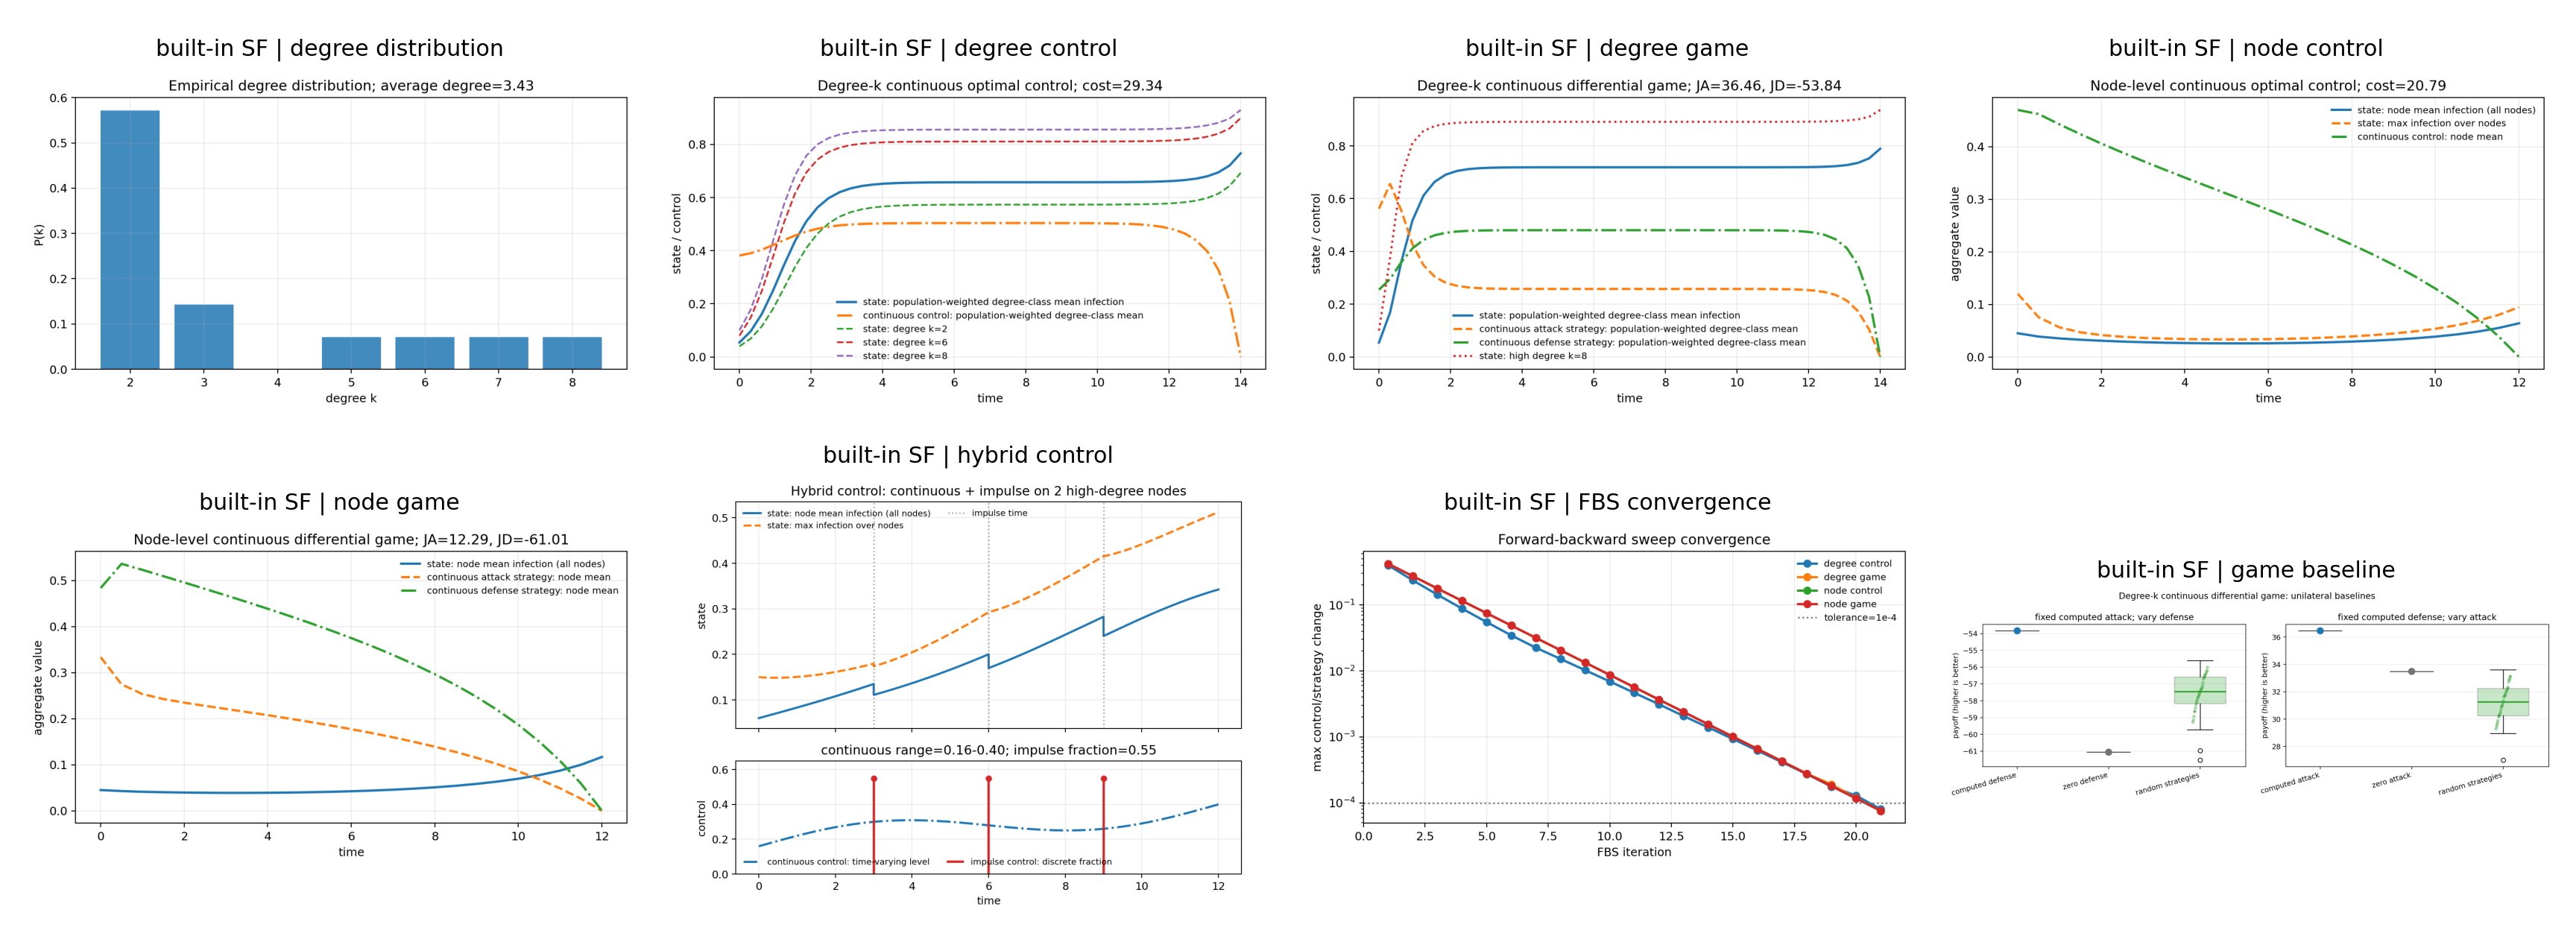
\includegraphics[width=0.92\textwidth]{../assets/foundation_examples_contact_sheet.png}
\caption{Visual index of the foundation examples, including degree-level control/game, node-level variants, convergence diagnostics, and hybrid impulse behavior.}
\label{fig:foundation-contact-sheet}
\end{figure}

\begin{figure}[p]
\centering
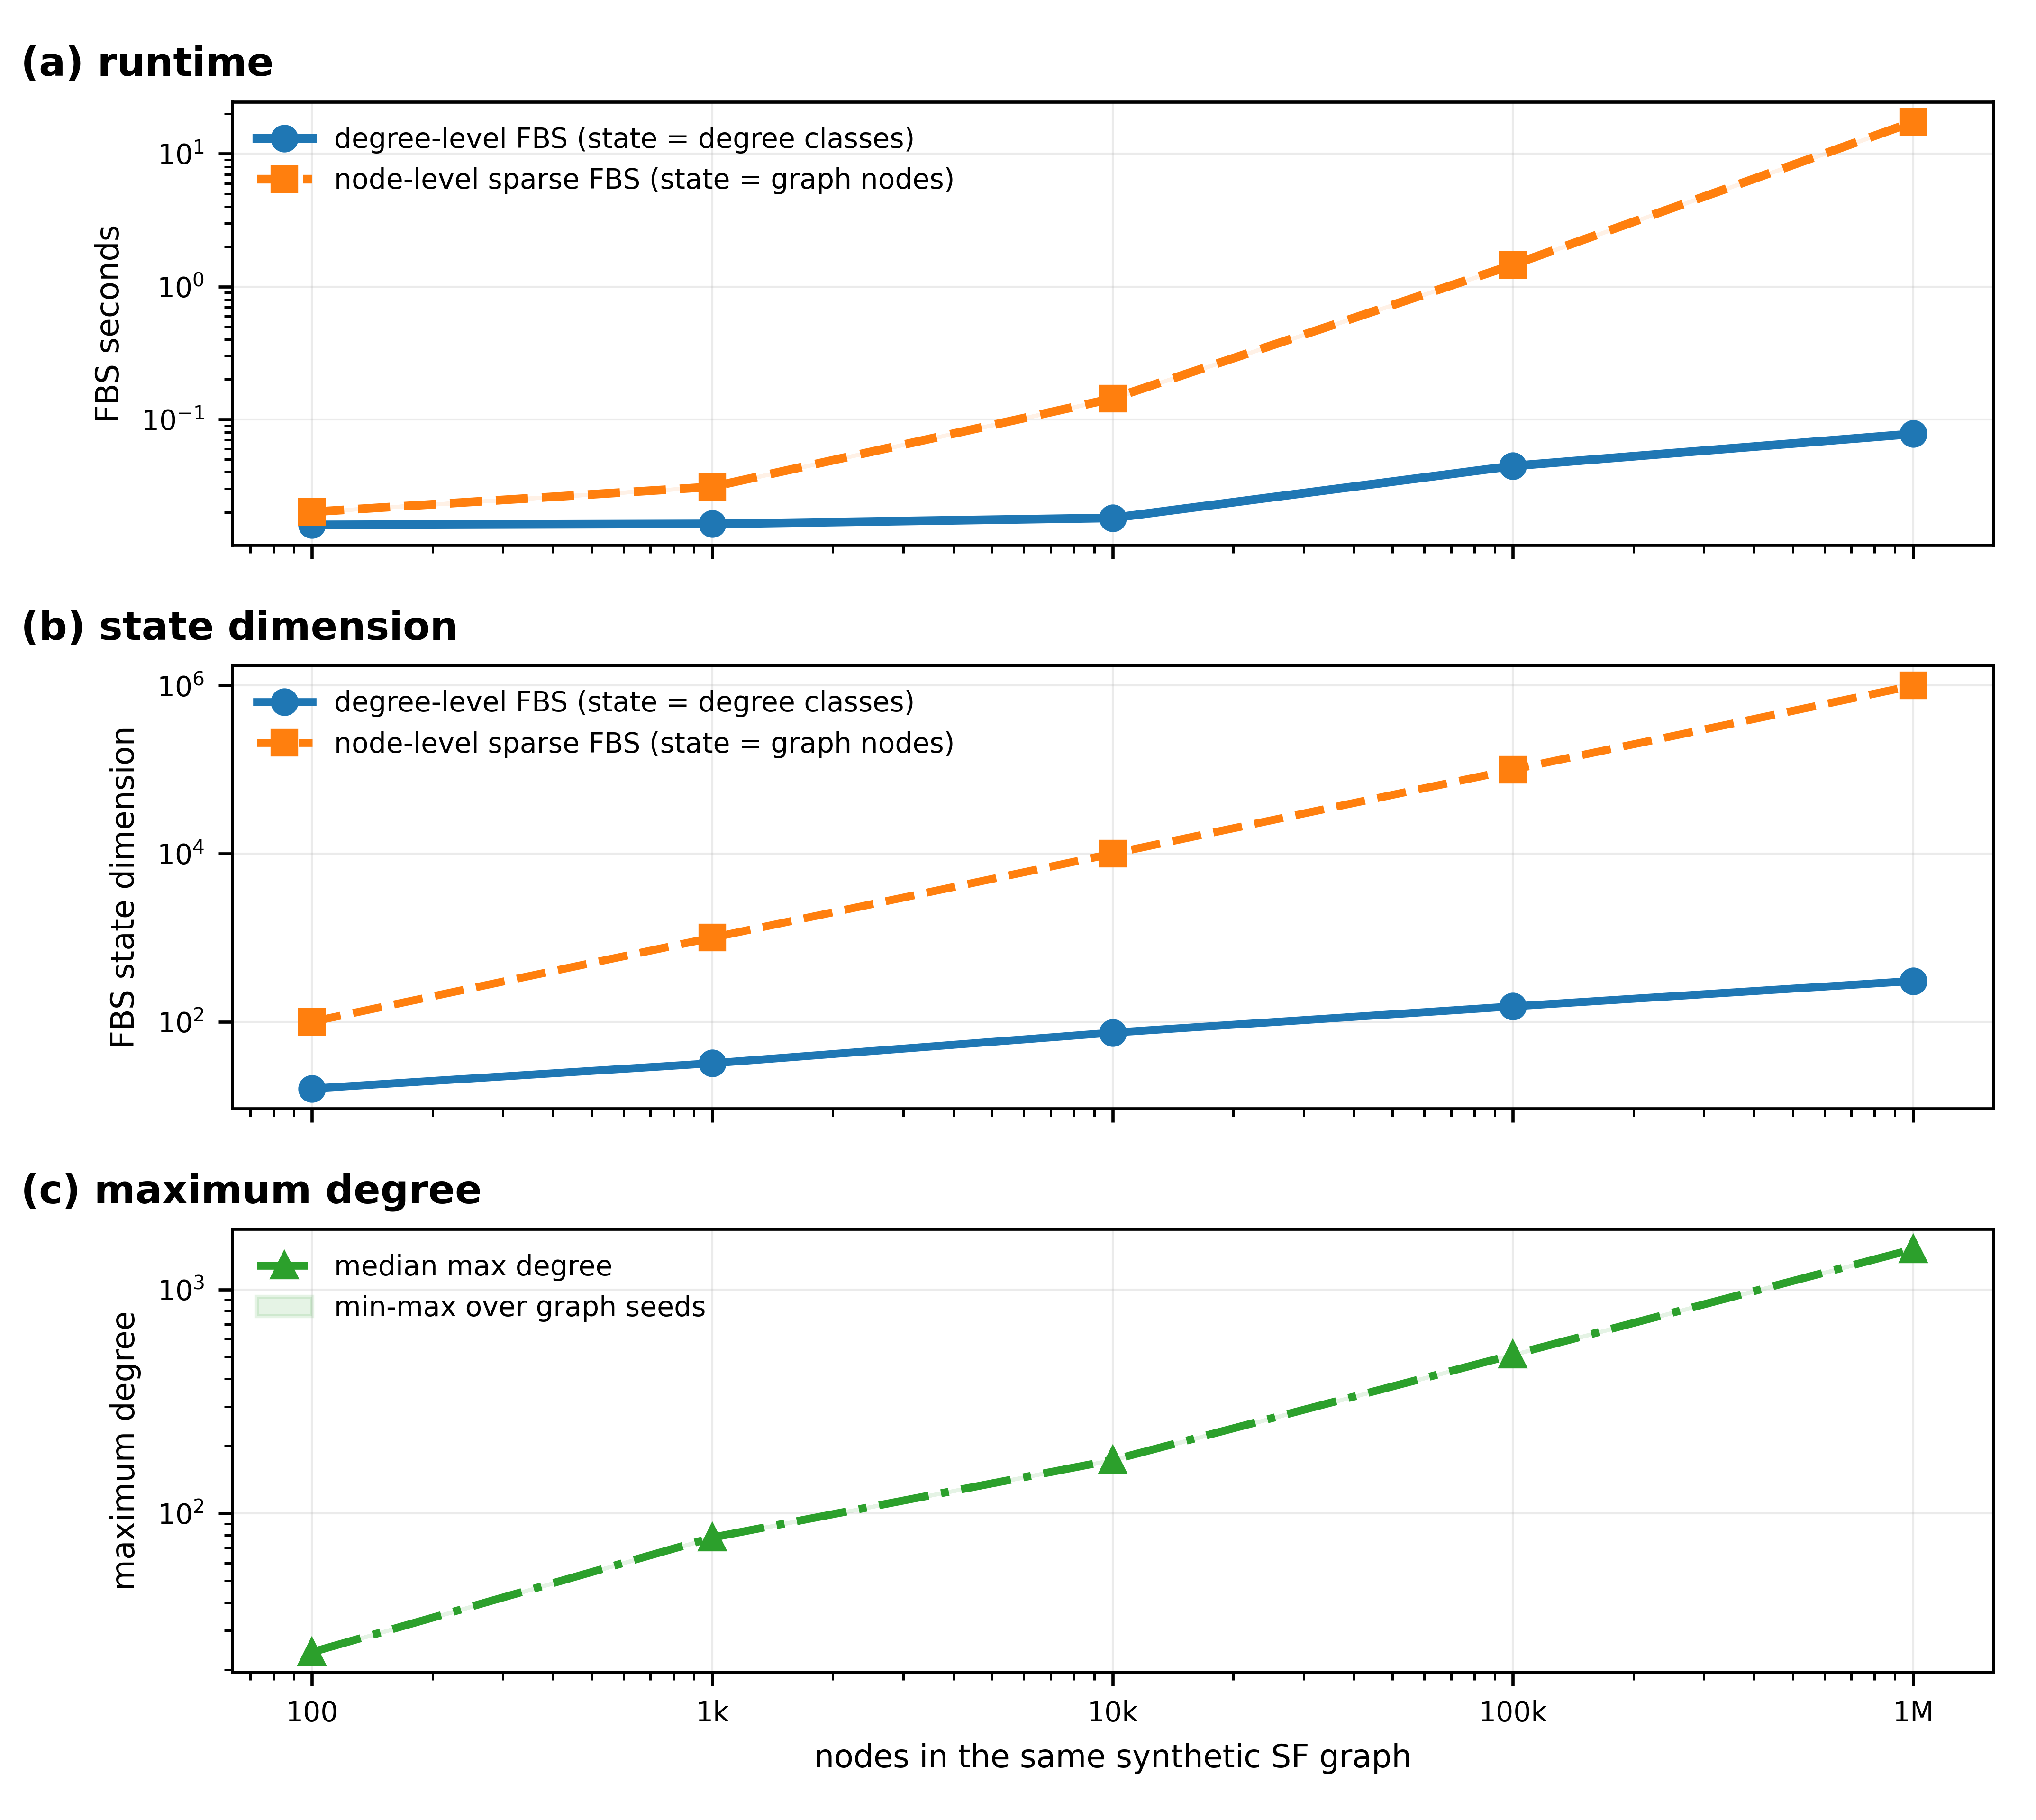
\includegraphics[width=0.92\textwidth]{../assets/degree_node_fbs_scalability.png}
\caption{Degree-level versus sparse node-level FBS timing on matched synthetic scale-free networks.}
\label{fig:degree-node-scalability}
\vspace{1em}
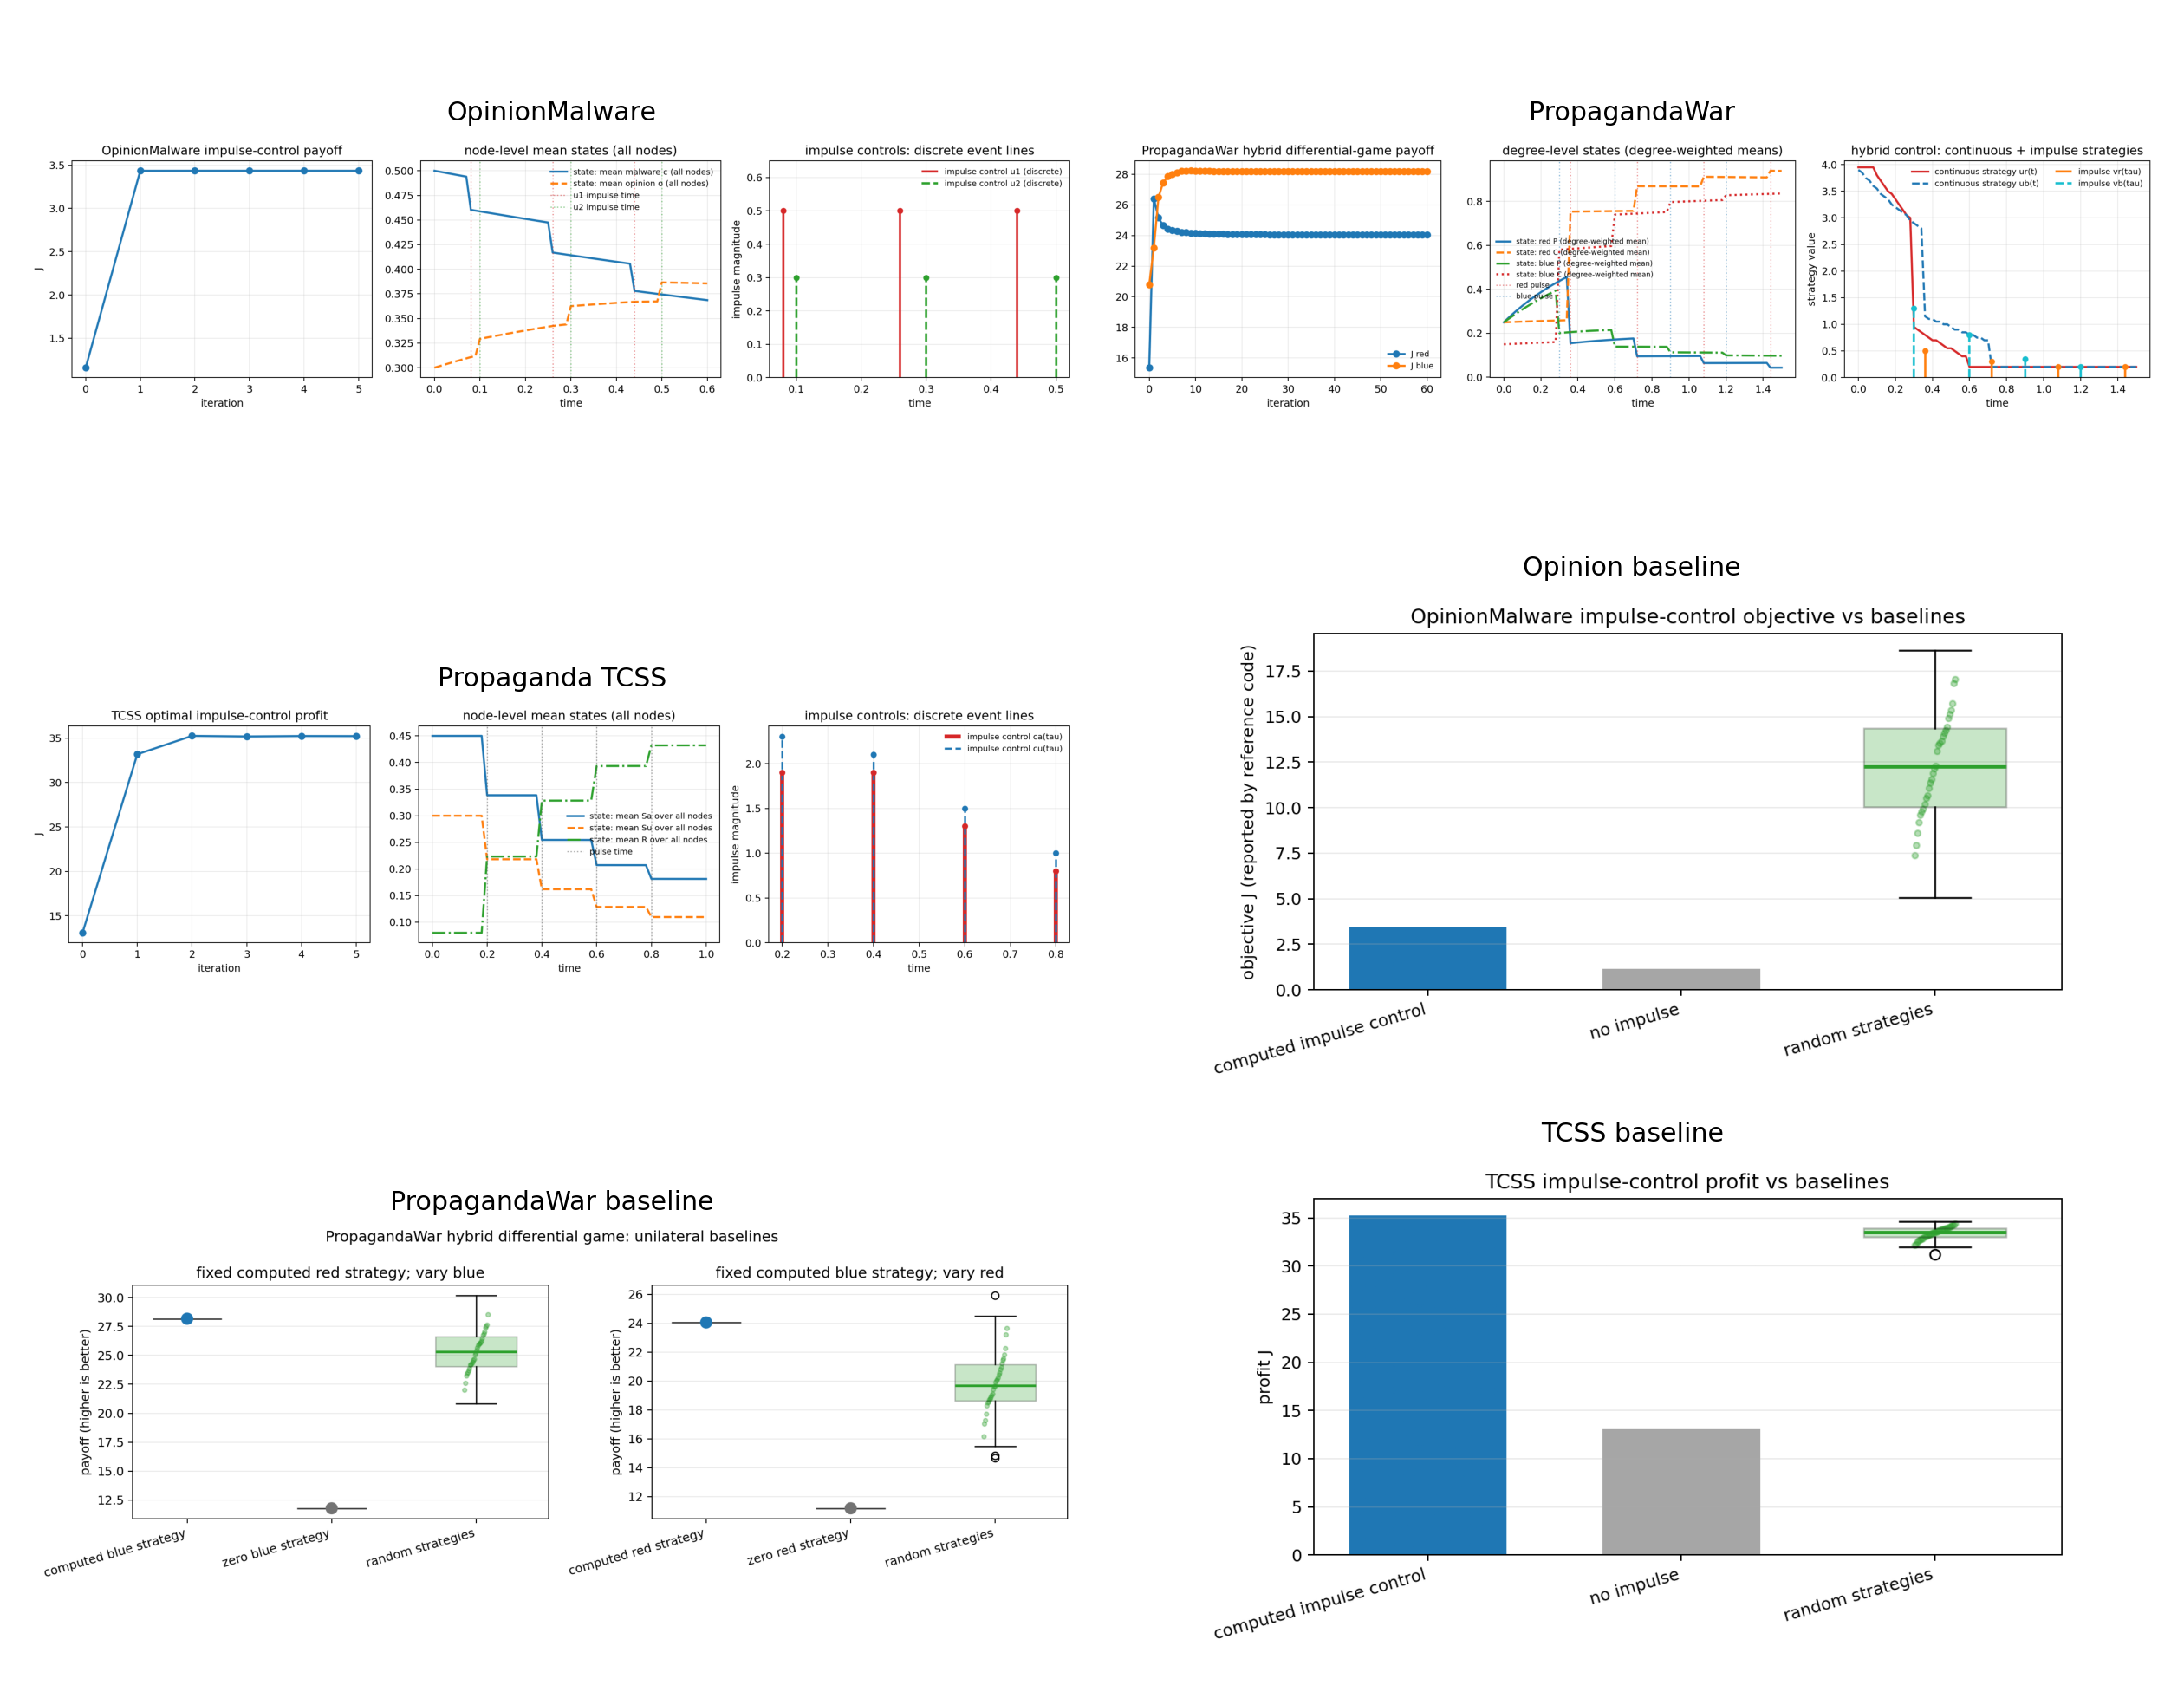
\includegraphics[width=0.92\textwidth]{../assets/reference_repo_contact_sheet.png}
\caption{Reference-repository smoke-run contact sheet for the paper-level code snapshots.}
\label{fig:reference-contact-sheet}
\end{figure}
\clearpage
% -----------------------------------------------------------------------------
\section{Glossary and References}
% -----------------------------------------------------------------------------

\subsection{Glossary}
\begin{longtable}{L{4.0cm}L{11.0cm}}
\toprule
\textbf{Term} & \textbf{Meaning} \\
\midrule
\endhead
State $x(t)$ & Variables describing the system at time $t$, such as node infection probabilities. \\
Control $u(t)$ & Decision variable chosen by a controller over time. \\
Payoff/cost functional $J$ & Cumulative objective over the time horizon. \\
Hamiltonian $H$ & Immediate payoff plus adjoint-weighted state dynamics. \\
Adjoint $\lambda(t)$ & Shadow value of the state; solved backward in time. \\
PMP & Pontryagin Maximum Principle; necessary conditions for optimal control or open-loop games. \\
HJB & Hamilton-Jacobi-Bellman equation; dynamic programming equation for feedback optimal control. \\
Nash equilibrium & Strategy profile where no player benefits from unilateral deviation. \\
Stackelberg equilibrium & Leader-follower equilibrium with sequential decision structure. \\
Impulse control & Discrete intervention causing instantaneous state jumps. \\
Hybrid control & Combination of continuous controls and impulses/switches. \\
Degree-level model & Model that groups nodes by degree/type rather than tracking each node. \\
Node-level model & Model that tracks each node and uses the adjacency matrix. \\
\bottomrule
\end{longtable}

\subsection{References and Source Notes}

\begin{enumerate}[label={[\arabic*]},leftmargin=2.1em]
  \item Isaacs, R. (1965). \emph{Differential Games}. John Wiley and Sons.
  \item Basar, T., and Zaccour, G. (eds.) (2018). \emph{Handbook of Dynamic Game Theory}. Springer.
  \item Simaan, M., and Cruz, J. B. (1973). Sampled-data Nash controls in non-zero-sum differential games. \emph{International Journal of Control}, 17(6), 1201-1209.
  \item Sadana, U., Reddy, P. V., and Zaccour, G. (2021). Nash equilibria in nonzero-sum differential games with impulse control. \emph{European Journal of Operational Research}, 295, 792-805.
  \item Yang, L.-X., Li, P., Yang, X., Xiang, Y., and Zhou, W. (2018). A differential game approach to patch injection. \emph{IEEE Access}, 6, 58924-58938.
  \item Yang, L.-X., Li, P., Zhang, Y., Yang, X., Xiang, Y., and Zhou, W. (2019). Effective repair strategy against advanced persistent threat: a differential game approach. \emph{IEEE Transactions on Information Forensics and Security}, 14(7), 1713-1728.
  \item Yang, L.-X., Huang, K., Yang, X., Zhang, Y., Xiang, Y., and Zhou, Y. Y. (2021). Defense against advanced persistent threat through data backup and recovery. \emph{IEEE Transactions on Network Science and Engineering}, 8(3), 2001-2013.
  \item Yang, L.-X., Li, P., Yang, X., and Tang, Y. Y. (2020). Simultaneous benefit maximization of conflicting opinions: modeling and analysis. \emph{IEEE Systems Journal}, 14(2), 1623-1634.
  \item Huang, D. W., Yang, L.-X., Li, P., Yang, X., and Tang, Y. Y. (2021). Developing cost-effective rumor-refuting strategy through game-theoretic approach. \emph{IEEE Systems Journal}, 15(4), 5034-5045.

  \item Cheng, X., Yang, L.-X., Li, G., Ma, Z., Zhu, T., Wang, L., and Duan, S. (2025). Modeling and Mitigating Social Engineering Malware: Integrating Malware-Opinion Dynamics With Optimal Impulse Control Approaches. Code repository: \url{https://github.com/XiaojuanCheng/OpinionMalware_TIFS_2025_Code}.
  \item Cheng, X., Yang, L.-X., Zhu, Q., Gan, C., Yang, X., and Li, G. (2024). Cost-Effective Hybrid Control Strategies for Dynamical Propaganda War Game. Code repository: \url{https://github.com/XiaojuanCheng/PropagandaWar_TIFS_2024_Code}.
  \item Cheng, X., Yang, L.-X., Zhu, Q., Gan, C., and Li, G. (2025). Impulse Strategies for Suppressing Cyber Propaganda With Awareness. Code repository: \url{https://github.com/XiaojuanCheng/Propaganda_TCSS_2025_Code}.
\end{enumerate}

\begin{sourcebox}{Source note}
This English tutorial note was consolidated from two uploaded source tutorial notes: a differential-game tutorial note and an optimal-hybrid-control tutorial note. The source materials cover the origins and classification of differential games, open-loop Nash differential games, Pontryagin-type optimality systems, forward-backward sweep, single-impulse games, hybrid control with state jumps, impulse Hamiltonians, and the nested optimization structure for impulse number, impulse times, and impulse magnitudes. The additional implementation sections translate these models into degree-level and node-level network workflows, including edge-list-to-adjacency conversion for realistic datasets, NetworkX/igraph graph support, ODE helper functions, and degree-distribution preprocessing for degree-$k$ models.
\end{sourcebox}


\appendix
\section{Tutorial Code Files}
\label{app:code}

The package contains the following runnable code and guide files:

\begin{itemize}
  \item \path{code/simple_degree_k_control.py}: minimal degree-$k$ optimal-control example.
  \item \path{code/network_control_examples.py}: main tutorial script for degree-level games, node-level models, and hybrid/impulse simulation.
  \item \path{README.md}: installation, commands, and usage notes.
  \item \path{reference_repository_guide.md}: mapping between the reference GitHub repositories and the mathematical workflow in this tutorial note.
  \item \path{../reference/download_reference_repositories.sh}: optional script to download the reference repositories.
\end{itemize}

\begin{lstlisting}[language=bash,caption={Core commands for the tutorial code.},numbers=none]
pip install -r requirements.txt

python code/simple_degree_k_control.py
python code/simple_degree_k_control.py \
  --edge-list sample_data/sample_edges.csv \
  --delimiter , --has-header --source-col source --target-col target

python code/network_control_examples.py
python code/network_control_examples.py --examples degree
python code/network_control_examples.py --adjacency-csv sample_data/sample_adjacency.csv

bash ../reference/download_reference_repositories.sh
\end{lstlisting}

This two-file code structure keeps the tutorial readable: the first script shows the degree-$k$ PMP logic, and the main tutorial script shows how the same logic extends to games, node-level adjacency models, and hybrid/impulsive interventions.

\end{document}
